% !TeX program = pdflatex
% Compile twice: pdflatex final_paper_llm_resume_audit.tex
\documentclass[10pt,twocolumn,letterpaper]{article}

\usepackage[utf8]{inputenc}
\usepackage[T1]{fontenc}
\usepackage{lmodern}
\usepackage{microtype}
\usepackage[margin=0.72in,columnsep=0.24in]{geometry}
\usepackage{setspace}
\setstretch{1.02}
\emergencystretch=2em
\hyphenpenalty=500
\tolerance=1500

\usepackage{amsmath,amssymb,mathtools,bm}
\usepackage{booktabs,tabularx,array,makecell}
\usepackage{graphicx}
\usepackage{xcolor}
\usepackage{enumitem}
\setlist{itemsep=1pt,topsep=2pt,leftmargin=*}
\usepackage{titlesec}
\titlespacing*{\section}{0pt}{0.75em}{0.35em}
\titlespacing*{\subsection}{0pt}{0.55em}{0.25em}
\titleformat{\section}{\large\bfseries}{\thesection}{0.5em}{}
\titleformat{\subsection}{\normalsize\bfseries}{\thesubsection}{0.45em}{}
\usepackage[colorlinks=true,linkcolor=blue!50!black,citecolor=blue!50!black,urlcolor=blue!50!black]{hyperref}

\title{\vspace{-1.4em}\textbf{When Algorithms Hire: Career-Stage Stratification in Large Language Model Resume Screening}}
\author{Yuheng Li\\Social Science and Data Mining}
\date{\vspace{-0.8em}May 2026}

\begin{document}
\maketitle

\begin{abstract}
Do large language models score resumes by qualification, identity, or labor-market status? I audit two Zhipu GLM screeners on 16,000 synthetic resume scores across 18 occupations, randomly assigning gender cues, U.S. name-origin cues, career stage, and objective-qualification blocks. Pooled gender and name-origin effects are small, and validation shows weak perception of some Black and Hispanic name cues by GLM 5.1. Career stage dominates: late-career applicants score 5.90 points and mid-career applicants 4.36 points above early-career applicants generated by the same instrument. LLM hiring audits should therefore examine career-stage stratification, model version, and occupation regime, not only aggregate gender/name-cue parity.
\end{abstract}

\section{Introduction}

Employers increasingly use automated systems to filter resumes before any human recruiter reads them. LLM-based screeners intensify the audit problem because they can read unstructured resumes and assign calibrated-looking scores, yet they are trained on labor-market text where qualification, identity, credentials, seniority, and status are entangled. A small scoring difference at this stage can scale into a large difference in access to interviews.

This paper asks a narrow causal question: holding the resume-generation process fixed, do implemented applicant cues change the score assigned by an LLM screener? I construct resumes from common templates and O*NET task statements, randomly assign gender, U.S. name-origin, career-stage, and objective-signal treatments, and submit the applications to GLM 5.1 and GLM 4.5 under a fixed scoring prompt. The design brings Bertrand and Mullainathan-style audit logic to an LLM decision-maker, covers a balanced 18-occupation panel, and treats name-based contrasts as implemented name-cue effects rather than direct race effects.

The main finding is not a large pooled gender/name-origin disparity. Those effects are small, and a validation check shows weak perception of some Black and Hispanic name cues by GLM 5.1. The strongest finding is career-stage stratification: mid- and late-career applicants are scored substantially above early-career applicants generated under the same audit instrument. I argue that this is a form of status translation. Experience can represent human capital, but it can also encode prior opportunity, stable employment histories, access to career ladders, and age-linked seniority. If an LLM learns these associations from labor-market text, it may convert career length into a general employability proxy. LLM hiring audits should therefore examine whether models reproduce hierarchy through signals that appear job-relevant, not only whether they react to protected-category cues.

\section{Research Design and Data}

\subsection{Factorial Audit}

The unit of design is a resume-treatment cell. A base resume $i$ is first generated for one of eighteen occupations. The resume is then assigned four randomized factors: gender signal $T_g \in \{\text{male},\text{female}\}$, U.S. name-origin cue $T_e \in \{\text{White},\text{Black},\text{Hispanic},\text{Asian}\}$, career-stage signal $T_p \in \{\text{early},\text{mid},\text{late}\}$, and an indicator $S$ for whether an explicit objective-qualification block is included. The resulting prompt is scored by model $M \in \{\text{GLM 5.1},\text{GLM 4.5}\}$. The outcome $Y$ is a 0--100 hiring score.

The realised design contains 8,000 treatment cells and 16,000 model-score observations. The occupation panel contains eighteen occupations arranged as a $3 \times 3 \times 2$ grid: gender stereotype (male, female, neutral) by skill tier (high, mid, low) by two occupations per cell. This construction avoids a common weakness of resume audits: all inference coming from a few occupations such as software engineering and nursing. The sample is stratified over occupation and factorial treatment cells, giving roughly nine replicates per occupation-treatment micro-cell.

The design deliberately separates three ideas that are often conflated in algorithmic-hiring debates. The first is the implemented cue: the textual information that allows a screener to infer gender, name-origin category, or career stage. The second is qualification content: occupation-specific tasks, education, experience, and credentials. The third is the decision environment: the job description and model used to evaluate the application. The experiment manipulates the first, controls the second within base-resume families, and stratifies the third. That separation is what allows the coefficients below to be interpreted as effects of implemented cues rather than as correlations between applicant groups and resume quality.

The resumes are synthetic but structured. Base resumes are generated from O*NET task taxonomies and templated with Faker and Jinja2 rather than produced by an LLM. This matters because LLM-generated prose could be recognized by the same class of model that later scores the resume. Names are drawn from a curated gender-by-name-origin corpus based on Census surname and first-name sources. Career stage is signaled through graduation years and experience histories. The objective-signal block includes GPA, certification identifiers, and standardized-test percentile information.

\begin{table*}[t]
\centering
\caption{Realised experimental design.}
\label{tab:design}
\begin{tabularx}{0.94\textwidth}{l X r}
\toprule
Component & Levels or source & Realised count \\
\midrule
Gender signal & male, female & 2 \\
U.S. name-origin cue & White/European American, African American, Hispanic/Spanish-Latin American, Asian/Vietnamese & 4 \\
Career-stage signal & early-career, mid-career, late-career & 3 \\
Objective-signal block & absent, present & 2 \\
Occupations & balanced stereotype $\times$ tier panel & 18 \\
Models & GLM 5.1 and GLM 4.5 via Zhipu paid API & 2 \\
Treatment cells & stratified sample from full factorial & 8,000 \\
Model-score observations & treatment cells $\times$ models & 16,000 \\
\bottomrule
\end{tabularx}
\end{table*}

\subsection{Name Cues and Estimand Scope}

The name-origin treatment should be read as a reduced-form name-cue intervention, not as an observation of race or ethnicity. The implemented surname bundle is Olson for White/European American, Washington for African American, Garcia for Hispanic/Spanish-Latin American, and Nguyen for Asian/Vietnamese cues, crossed with gendered first names. Random assignment identifies the effect of assigning this bundle to an otherwise controlled resume prompt. It does not identify how the model would respond to race observed directly, to photos, to self-identification, or to a different name set.

This distinction matters empirically. A separate 192-call validation check asked both GLM models to classify the intended U.S. name-cue origin of the 32 full names, with three repeats per name-model pair. GLM 4.5 recognized the cues well overall (94.8 percent accuracy), but GLM 5.1 frequently returned ``unclear'' for Washington and Garcia names: Black-name accuracy was 8.3 percent with a 91.7 percent unclear rate, and Hispanic-name accuracy was 20.8 percent with a 75.0 percent unclear rate. The main tables therefore report score-level responses to implemented gender and name-origin cues. Weak Black and Hispanic coefficients should be interpreted partly through this measurement first stage.

\subsection{Model Panel}

The main panel uses GLM 5.1 and GLM 4.5 through the Zhipu paid API. The original design considered a wider model roster, but pre-flight diagnostics showed that several free-tier alternatives collapsed the score distribution into only a few unique values under the calibrated prompt. Including such models would have made continuous-score regression and CATE estimation difficult to interpret. Details of this panel-trimming step are reported in Appendix~\ref{app:preexp}. The cost is a narrower external-validity claim: the results apply to this GLM family and should not be generalized mechanically to OpenAI, Anthropic, Workday, or Eightfold systems.

The scoring prompt asks the model to act as a first-pass resume screener and return a hiring score on a 0--100 scale. The prompt does not tell the model that the audit concerns applicant-cue sensitivity and does not label the treatments. This reduces demand effects: if the model were explicitly told that names or career-stage cues were being audited, the desired behavior would be obvious. The design instead embeds the treatment in an ordinary screening task and tests whether the model uses it.

\section{Identification and Estimation}

\subsection{Potential Outcomes}

Let $Y_i(t)$ denote the score that base resume $i$ would receive if assigned implemented cue value $t$. The estimand for a binary treatment contrast is
\[
\tau(t,t') = \mathbb{E}[Y_i(t)-Y_i(t')].
\]
For name-origin and career-stage cues, the baseline categories are White and early-career respectively. The experiment observes one realised treatment condition for each cell, but random assignment ensures that observed differences in conditional means identify average potential-outcome differences. The formal proof is given in Appendix~\ref{app:proofs}; the core argument is that the random number generator, not resume quality, determines treatment.

This gives strong internal validity for the audit instrument. Treatment assignment is independent of latent resume quality, and every treatment level has positive probability in every design stratum. Consistency is also plausible because each treatment is a concrete string manipulation: a name replacement, a career-stage signal, and a qualification block. The main remaining dependence is repeated use of the same base resumes, which motivates cluster-robust standard errors by base resume.

External validity is weaker. A score is not a callback, synthetic resumes are not real applicants, and two Zhipu models are not the market for hiring AI. The audit should therefore be read as a controlled test of applicant-cue sensitivity in one LLM family, not as a direct estimate of employer behavior. Its value is internal validity: randomization, complete control over resume content, and replication of the same instrument across models.

\subsection{OLS, CATE, and Multiple Testing}

The primary model is
\begin{align}
Y_{ijm} ={}& \alpha + \beta_g T^g_i + \bm{\beta}_e^\top T^e_i
 + \bm{\beta}_p^\top T^p_i + \beta_S S_i \nonumber\\
&+ \delta_j + \mu_m + \varepsilon_{ijm},
\end{align}
where $\delta_j$ are occupation fixed effects and $\mu_m$ are model fixed effects. Standard errors are clustered at the base-resume level. Because implemented cue factors are randomized, fixed effects are used for precision and design accounting, not for confounding adjustment.

To estimate heterogeneity, I fit generalized random forests for each non-baseline contrast and report the 1st, 50th, and 99th percentiles of the estimated CATE distribution. These estimates are descriptive maps of heterogeneity rather than replacement estimators for the main ATE. Finally, family-wise error is controlled using a Romano-Wolf/List-Shaikh-Xu style step-down correction over 21 contrasts: seven implemented-cue coefficients across the full panel, GLM 5.1, and GLM 4.5.

The estimation strategy is hierarchical. OLS supplies the primary causal estimates because it follows directly from the randomized design. The CATE analysis answers where the pooled effect is misleading, not whether the pooled design is identified. Multiple-testing correction disciplines the interpretation of many cue contrasts. Robustness checks then ask whether the results depend on a merge pipeline, scoring format, or retrieval period.

\section{Results}

\subsection{Pooled Average Effects}

Table~\ref{tab:ols} reports the main pooled OLS coefficients. The pooled gender and name-origin cue effects are small in score units. Female names receive a 0.220 point premium relative to male names. Asian/Vietnamese name cues receive a 0.373 point penalty relative to White/European American cues. Black and Hispanic name-cue coefficients are also negative, at -0.197 and -0.146, but are not statistically distinguishable from zero. The female and Asian coefficients have raw $p$-values near 0.03, but their family-wise adjusted $p$-values are both 0.089, so they do not survive the registered correction in the full panel.

These effect sizes are small relative to the 0--100 scale. A 0.22 point female premium is unlikely to change a hiring decision if the score is used literally and downstream thresholds are coarse. However, small score shifts can matter when automated pipelines rank many similar applicants near a cutoff, and their importance depends on how employers map scores into interview decisions. The correct interpretation is therefore bounded: the pooled panel does not show a large gender or name-origin penalty, but it also does not prove that gender and race would be irrelevant under other signals, modalities, or operational screening systems.

The career-stage effects are much larger. Late-career applicants score 5.903 points above early-career applicants generated under the same occupation-specific audit instrument, and mid-career applicants score 4.364 points higher. Both survive family-wise correction easily. In practical terms, career stage is the largest cue dimension in the audit. It is also more robust than gender or name-origin cues, appearing strongly in both models and across the CATE distribution.

This result is not automatically evidence of a legal violation. Many jobs legitimately value experience, and the treatment bundle includes years of experience as part of the career-stage signal. The social-science question is sharper: is the model evaluating current job capacity, or is it treating career length as a legitimate status signal? In this audit, career stage bundles age, accumulated work years, occupational stability, and the culturally familiar image of a mature candidate. The model's score premium may therefore reflect a seniority premium learned from labor-market text rather than only a direct assessment of task competence. If an employer intends to evaluate minimum qualifications or current job fit, such a strong career-stage premium could become a mechanism of score-level stratification.

The objective-signal coefficient reverses the preregistered expectation: the credential block lowers the score by 0.252 points and survives the family-wise correction at 0.042. This is not evidence that objective information harms applicants. The generated GPA has a mean around 3.42, which appears mediocre in high-tier occupations such as lawyers and financial analysts. The result is better read as a design lesson: ``objective'' signals must be normed to occupational expectations before they can serve as cue-reducing anchors.

\begin{table*}[t]
\centering
\caption{Pooled OLS implemented-cue coefficients. Outcome is 0--100 hiring score; standard errors are clustered by base resume. FWER values come from the 21-contrast step-down correction. Source: OLS, MHT output tables.}
\label{tab:ols}
\begin{tabular}{lrrrr}
\toprule
Coefficient & Estimate & SE & raw $p$ & FWER $p$ \\
\midrule
Female cue & 0.220 & 0.103 & 0.033 & 0.089 \\
Asian/Vietnamese cue & -0.373 & 0.175 & 0.034 & 0.089 \\
African American cue & -0.197 & 0.143 & 0.168 & 0.418 \\
Hispanic/Spanish-Latin cue & -0.146 & 0.138 & 0.289 & 0.532 \\
Late-career & 5.903 & 0.174 & $<10^{-100}$ & 0.001 \\
Mid-career & 4.364 & 0.173 & $<10^{-100}$ & 0.001 \\
Objective signal present & -0.252 & 0.107 & 0.019 & 0.042 \\
\bottomrule
\end{tabular}
\end{table*}

\subsection{Within-Vendor Model Contrast}

The pooled results mask an important model contrast. In the multiple-testing table, GLM 5.1 shows significant female and Asian/Vietnamese name-cue sensitivity after correction: the female contrast has adjusted $p=0.011$, and the Asian contrast has adjusted $p=0.010$. GLM 4.5 is neutral on every implemented cue axis; its smallest adjusted $p$ among the gender/name-origin contrasts is far from conventional significance. Since the prompt, resume pool, outcome scale, and vendor family are held fixed, this is a within-vendor model-version contrast rather than a cross-provider comparison.

The direction is also notable. The significant GLM 5.1 gender result is a female premium, not the female penalty one might expect from the human callback literature. The Asian/Vietnamese name-cue result is a penalty. Thus the audit does not simply reproduce Bertrand and Mullainathan in LLM form. It instead shows that implemented-cue sensitivity exists in some model settings, but its direction and affected groups can differ from traditional human-employer baselines.

This point matters for audit policy. A compliance procedure that certifies one model version and assumes nearby versions behave similarly could miss changes induced by model upgrades. Conversely, a result on one model snapshot should not be attributed automatically to another model from the same provider. The present two-model design cannot explain why GLM 5.1 is more sensitive on these axes. Possible mechanisms include stronger semantic extraction, different alignment behavior, or greater use of social associations embedded in resume names. The contribution is narrower but still important: model version is an audit-relevant factor.

\subsection{Heterogeneity}

Table~\ref{tab:cate} reports CATE percentile spreads. These estimates support the second hypothesis: implemented-cue effects vary by occupation and model. For the female contrast, the CATE distribution runs from -3.30 at the 1st percentile to +4.62 at the 99th percentile. The mean is close to the pooled OLS coefficient, but the tails imply that some occupation-model cells experience meaningfully different gender-cue effects.

Name-origin cues show the same pattern. The Asian/Vietnamese contrast has a mean of -0.43 but a 1st percentile of -9.06, indicating that a small slice of occupation-model cells concentrates a much larger penalty. Black and Hispanic name-cue effects have means near zero, but their percentile spreads cover roughly eight score points. These patterns are important for audit practice: a pooled null can coexist with substantial conditional cue responses in specific labor-market segments.

Career stage again dominates. The late-career CATE distribution has a median of 6.09 and a 99th percentile of 17.33. Mid-career has a median of 4.03 and a 99th percentile of 12.97. These are not merely statistically detectable differences; they are large relative to the 0--100 scale and to the gender/name-origin coefficients.

The CATE results clarify why a single headline coefficient is inadequate for an audit. If a regulator, employer, or model vendor reports only pooled gender/name-origin averages, the report may miss where implemented-cue sensitivity is operationally concentrated. A job-category fixed effect controls average differences across occupations; it does not reveal whether the cue contrast itself changes by occupation. The forest estimates are therefore best read as a map for follow-up inspection. They identify where a human auditor should examine prompts, rationales, and job-specific scoring rules more closely.

The forest results motivate a more interpretable regime-level analysis, reported next. Rather than treating heterogeneity as a black-box percentile spread, I aggregate occupations into the pre-specified stereotype-by-tier regimes and ask where the cue responses are concentrated.

\begin{table*}[t]
\centering
\caption{CATE percentile spreads from generalized random forests. Source: CATE output table.}
\label{tab:cate}
\begin{tabular}{llrrrrr}
\toprule
Axis & Contrast & $n$ & $p_{01}$ & $p_{50}$ & $p_{99}$ & Mean \\
\midrule
Gender & Female & 16,000 & -3.30 & 0.14 & 4.62 & 0.23 \\
Name-origin & Asian/Vietnamese & 7,990 & -9.06 & -0.13 & 3.15 & -0.43 \\
Name-origin & African American & 7,994 & -4.20 & -0.11 & 4.53 & -0.11 \\
Name-origin & Hispanic/Spanish-Latin & 8,016 & -4.10 & -0.20 & 4.16 & -0.21 \\
Career stage & Late-career & 10,656 & -1.08 & 6.09 & 17.33 & 5.90 \\
Career stage & Mid-career & 10,670 & -1.33 & 4.03 & 12.97 & 4.31 \\
\bottomrule
\end{tabular}
\end{table*}

\subsection{Hiring Regimes and Transportability}

The 18 occupations can also be read as nine observable hiring regimes: occupation gender stereotype crossed with skill tier. This is not a firm-level employer heterogeneity estimate. I do not observe employer culture, recruiter preferences, or deployed applicant-tracking rules. Instead, the regime analysis asks whether the same randomized audit effect changes across observable role environments that real employers hire into.

Table~\ref{tab:regime} estimates the OLS specification separately inside each stereotype-by-tier regime, retaining occupation and model fixed effects. The pooled female coefficient of about +0.22 is not stable across regimes: it is +1.21 in male-typed high-skill roles but -0.41 in male-typed mid-skill roles. The Asian/Vietnamese name-cue coefficient is most negative in female-typed high-skill roles (-1.54), while several low- and mid-skill regimes are close to zero. Career-stage premiums remain positive in every regime, ranging from +3.14 to +8.88 for late-career and from +2.23 to +6.46 for mid-career. The objective-signal penalty is concentrated in high-skill roles, especially female-typed high-skill roles (-1.75), which is consistent with the GPA-calibration explanation above.

\begin{table*}[t]
\centering
\caption{Role-regime OLS coefficients. Each row fits the main OLS within one stereotype-by-tier regime, with occupation and model fixed effects retained. Source: \texttt{role\_regime\_heterogeneity.csv}.}
\label{tab:regime}
\scriptsize
\begin{tabular}{llrrrrrrr}
\toprule
Stereotype & Tier & Female & Asian/Viet. & Afr. Am. & Hisp./Lat. & Mid-career & Late-career & Obj. signal \\
\midrule
Male & High & +1.209 & -0.283 & -0.505 & -0.247 & +6.119 & +7.087 & -0.188 \\
Male & Mid & -0.408 & -0.384 & -0.016 & -0.266 & +5.315 & +7.025 & +0.362 \\
Male & Low & -0.031 & +0.023 & +0.227 & +0.121 & +4.915 & +5.966 & -0.073 \\
Female & High & +0.273 & -1.540 & -0.064 & +0.892 & +6.456 & +8.877 & -1.751 \\
Female & Mid & -0.116 & -0.338 & -0.158 & -0.219 & +2.232 & +3.135 & -0.678 \\
Female & Low & +0.193 & -0.168 & -0.416 & -0.517 & +3.919 & +5.897 & +0.468 \\
Neutral & High & +0.257 & -0.302 & +0.201 & -0.394 & +4.381 & +6.285 & -0.433 \\
Neutral & Mid & +0.275 & -0.294 & -0.802 & -0.955 & +3.053 & +4.936 & +0.103 \\
Neutral & Low & +0.330 & -0.091 & -0.279 & +0.210 & +2.892 & +3.938 & -0.061 \\
\bottomrule
\end{tabular}
\end{table*}

This matters for external validity because the headline pooled coefficient is a balanced-audit estimand. Real hiring markets have different mixes of occupations and employers. Table~\ref{tab:transport} reweights the nine regime effects under six market compositions. BLS/OES employment weights barely change gender/name-origin estimates relative to the balanced audit. But a high-skill professional market would imply a more negative Asian/Vietnamese name-cue effect (-0.91, a -0.53 transportability gap) and larger career-stage premiums; a service/manual market would attenuate the Asian/Vietnamese penalty to -0.18 and reduce late-career effects by about 1.13 points. Thus the study should not be read as estimating a universal labor-market average. It estimates the balanced audit panel, and transport to a real employer mix depends on the composition of roles being screened.

\begin{table*}[t]
\centering
\caption{Employer-mix transportability sensitivity. Entries are reweighted effects; parentheses are gaps relative to the balanced-audit market. Source: \texttt{transportability\_sensitivity.csv}.}
\label{tab:transport}
\scriptsize
\begin{tabular}{lrrrr}
\toprule
Market composition & Female & Asian/Viet. & Late-career & Objective signal \\
\midrule
Balanced audit & +0.220 (+0.000) & -0.375 (+0.000) & +5.905 (+0.000) & -0.250 (+0.000) \\
BLS/OES employment-weighted & +0.241 (+0.021) & -0.394 (-0.019) & +5.650 (-0.255) & -0.327 (-0.077) \\
High-skill professional & +0.533 (+0.313) & -0.907 (-0.532) & +7.790 (+1.885) & -1.014 (-0.764) \\
Service/manual & +0.121 (-0.099) & -0.184 (+0.191) & +4.773 (-1.132) & -0.046 (+0.204) \\
Male-typed & +0.302 (+0.081) & -0.157 (+0.219) & +6.539 (+0.634) & -0.026 (+0.224) \\
Female-typed & +0.120 (-0.100) & -0.833 (-0.458) & +6.246 (+0.341) & -0.912 (-0.661) \\
\bottomrule
\end{tabular}
\end{table*}

\begin{figure}[t]
\centering
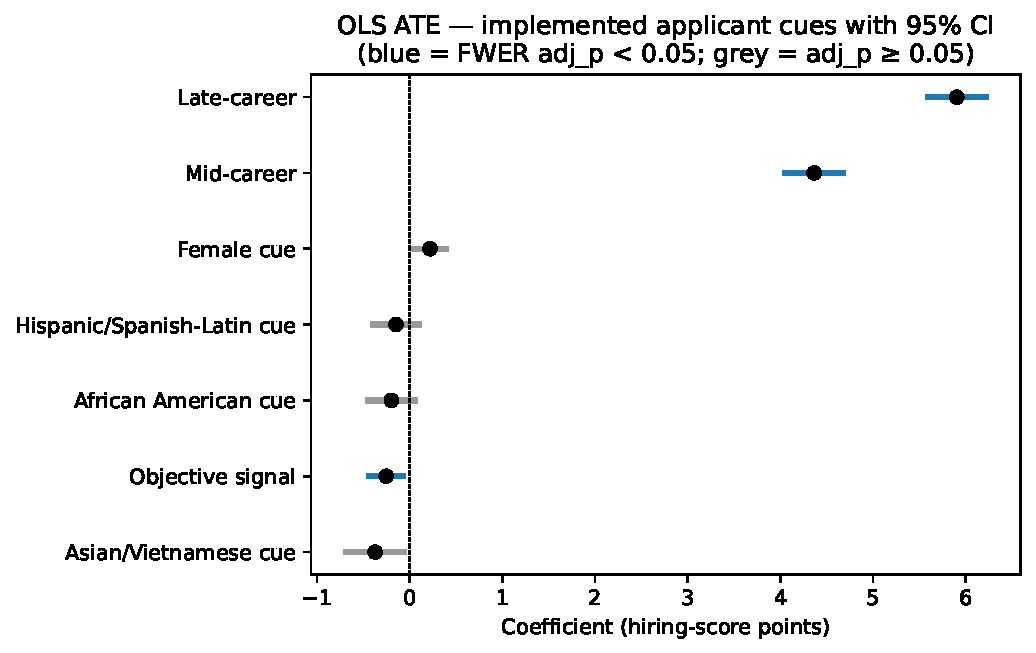
\includegraphics[width=\columnwidth]{../figures/forest.pdf}
\caption{Forest plot of implemented-cue OLS coefficients with 95 percent intervals. Source: reporting output.}
\label{fig:forest}
\end{figure}

\section{Robustness}

Table~\ref{tab:robust} summarizes the robustness checks. The first is a within-cluster permutation placebo. Treatment labels are shuffled within each base-resume cluster and the OLS model is refit 500 times. If the main results were driven by a merge error or leakage from resume identity into treatment assignment, the placebo distribution would not be centered near zero. The test passes this diagnostic: all placebo means are within $\pm 0.5$ score points. Career-stage, Asian/Vietnamese name-cue, and objective-signal coefficients fall in the tails of their placebo distributions, while Black and Hispanic name-cue coefficients do not, matching the main inference.

The second robustness check changes the elicitation format. A subsample is scored with a ranking prompt: the model sees five candidates for the same job and ranks them from best to worst. The ranking is converted to a 0--100 Borda score and the OLS model is refit. The realised Borda sweep contains 990 cells, or 198 five-candidate groups evaluated by two Zhipu models. Five of seven coefficient directions match the direct-score design: career-stage contrasts remain positive and all name-origin cue coefficients remain negative. Female and objective-signal coefficients flip. Because Borda standard errors are large, around 1.7--2.7 score points, this is evidence of partial directional robustness rather than a powered replication.

The third check addresses temporal drift. The 16,000 scored observations are split into three retrieval windows, and the implemented-cue coefficients are re-estimated in each. Female and name-origin coefficients remain within 0.81 score points max-min across windows. Career-stage coefficients vary by 1.22--1.35 points but remain strongly positive. Thus the headline result is not an artifact of one retrieval period.

Together, the robustness checks support a cautious conclusion. The career-stage premium is stable across placebo, Borda, and temporal checks. The Asian/Vietnamese name-cue penalty is directionally supported in the Borda sweep and appears in the placebo tail, but its pooled family-wise significance is marginal. The female result is the most format-sensitive: it is positive under direct scoring and negative under Borda. That instability is one reason the paper avoids claiming a general female advantage or disadvantage. The robust claim is instead about score-level career-stage stratification, model-specific sensitivity, and heterogeneity.

\begin{table*}[t]
\centering
\caption{Robustness checks. Source: placebo, Borda, and temporal drift output tables.}
\label{tab:robust}
\begin{tabularx}{0.94\textwidth}{l X}
\toprule
Check & Main conclusion \\
\midrule
Permutation placebo & All placebo means within $\pm0.5$; no merge-leak signature. Asian name-cue, career-stage, and objective-signal effects are in placebo tails. \\
Borda ranking sweep & 990 cells; 5/7 signs match direct-score OLS. Career-stage and name-origin directions persist; female and objective signal flip with large SEs. \\
Temporal drift & Three retrieval windows show no implemented-cue reversal; career-stage premiums remain positive in every window. \\
Deferred checks & Open-vs-commercial contrast is infeasible under the locked single-vendor panel; photo extension requires a multimodal path and face assets. \\
\bottomrule
\end{tabularx}
\end{table*}

\section{Discussion}

The audit's strongest substantive finding is not a gender or name-origin coefficient, but career-stage stratification. Late-career and mid-career signals raise scores by several points even after holding the resume-generation process fixed. This may reflect a reasonable preference for experience, but it also shows how an LLM screener can convert career length into an apparently legitimate score advantage. In social-science terms, career stage is not just an age variable. It bundles human-capital accumulation, labor-market signaling, credentialized seniority, occupational stability, and statistical expectations about what a mature candidate should look like.

This interpretation changes the center of the paper. The audit does not show a large pooled gender/name-origin penalty in this GLM panel. It does show that the model rewards a status-laden signal that is often treated as job-relevant. That is a subtler mechanism of algorithmic stratification. A screener can reproduce labor-market hierarchy without directly using protected categories if it strongly privileges signals that encode seniority, stability, and prior opportunity. The present design cannot determine whether the premium is appropriate for any particular job, but it identifies where a governance question should begin: is the model measuring current job fit, or is it importing a broad seniority premium from labor-market text?

The second finding is that model version may matter. GLM 5.1 shows implemented-cue sensitivity that GLM 4.5 does not. This should be interpreted cautiously. A two-model within-vendor contrast cannot establish a universal law that larger models are more sensitive to applicant cues. It does show, however, that audits should not treat all versions of a vendor's model family as interchangeable. A compliance audit tied to one model snapshot may not transfer to another.

The third finding concerns the value of controlled synthetic audits relative to traditional methods. Compared with observational hiring data, this design has much stronger internal validity: the implemented cue is randomized, the resume content is held fixed, and every coefficient has a clear intervention interpretation. Compared with human callback audits, it is cheaper, scalable, and can test many occupation-model cells quickly. The cost is ecological validity. LLM scores are not human callbacks, and synthetic resumes may miss features of real applicant pools. The best use of this design is therefore as a diagnostic layer: it identifies whether a model is sensitive to implemented applicant cues under controlled conditions, after which field validation can test whether the same pattern appears in real hiring pipelines.

This diagnostic use has practical implications. Employers adopting LLM screeners should not rely only on vendor-wide fairness statements or aggregate benchmark performance. They should run occupation-specific audits using the actual scoring prompt and model version deployed in the workflow. They should report career-stage contrasts alongside gender and name-cue contrasts. They should also treat objective-qualification features as design objects: if the feature is poorly calibrated to occupation, it can introduce noise or unintended penalties rather than reduce cue reliance.

\section{Limitations and Conclusion}

Several limitations bound the claims. First, the model panel is restricted to two Zhipu GLM models. Free-tier comparators were excluded because they did not produce sufficiently granular scores, and OpenAI/Anthropic systems were excluded on cost and API-scope grounds. Second, the OSF lock was delayed until after the main batch. The design instrument was fixed before scoring and the analysis protocol follows the written proposal, but the registration timing is not ideal. Third, the outcome is a score, not a callback, interview, or offer. Fourth, the objective-signal block was not calibrated tightly enough to occupation tier; the negative signal coefficient is therefore a design lesson rather than a general finding about credentials.

\subsection{Name-Cue Measurement Validity}

As noted in the research design, name-origin is implemented through U.S. name cues, not observed race. I therefore ran a 192-call manipulation check: 32 audit names were classified by both GLM models with three repeats each under a resume-audit codebook asking for the intended U.S. name-cue origin. GLM 4.5 recognized the cues well overall, with 94.8 percent accuracy and no unclear responses. GLM 5.1 recognized Asian cues perfectly and White cues in 83.3 percent of repeats, but it frequently marked Washington and Garcia names as unclear. For GLM 5.1, Black-name accuracy was 8.3 percent with a 91.7 percent unclear rate, and Hispanic-name accuracy was 20.8 percent with a 75.0 percent unclear rate.

\begin{table*}[t]
\centering
\caption{Name-cue validation by model and intended name-origin category. Entries are accuracy / unclear rate over 24 repeats per cell. Source: \texttt{name\_signal\_validation\_full\_summary.csv}.}
\label{tab:namevalid}
\scriptsize
\begin{tabular}{lrrrrr}
\toprule
Model & White/Euro. & Afr. Am. & Hisp./Lat. & Asian/Viet. & Overall \\
\midrule
GLM 5.1 & .833 / .167 & .083 / .917 & .208 / .750 & 1.000 / .000 & .531 \\
GLM 4.5 & 1.000 / .000 & .792 / .000 & 1.000 / .000 & 1.000 / .000 & .948 \\
\bottomrule
\end{tabular}
\end{table*}

This result narrows interpretation. The name-origin coefficients are effects of the implemented name-cue bundle (Olson, Washington, Garcia, Nguyen), not effects of race as a directly observed social category. High ``unclear'' rates also imply classical attenuation for the intended contrast if the model sometimes does not perceive the cue. Thus the weak Black and Hispanic coefficients should not be read as evidence that race would be irrelevant under clearer or multimodal signals. They are evidence that these textual name cues produced little score movement in this GLM audit.

Within those limits, the study demonstrates that a factorial LLM audit can deliver clean causal evidence about implemented-cue sensitivity. In this GLM panel, pooled gender/name-origin cue effects are small and mostly do not survive family-wise correction, but GLM 5.1 alone shows female and Asian/Vietnamese name-cue sensitivity. Career-stage premiums are large, robust, and practically meaningful. Heterogeneity is substantial enough that pooled averages understate score-level disparities in particular occupation-model cells. Future audits should extend the same instrument to more vendors, real HR evaluators, and callback-like outcomes.

The broader conclusion is methodological. LLM hiring systems can be audited with the same causal logic used in human audit studies, but the scale and controllability of model calls allow a richer factorial design. That design does not eliminate the need for field validation. It does, however, provide a disciplined first test: if a model reacts to applicant cues when the resume instrument is held fixed, employers and regulators have a concrete reason to inspect deployment more closely.

For a final deployment audit, the next step would be validation against human recruiters or real platform outcomes. The synthetic audit can say that a model score changes under a controlled intervention; it cannot say how an employer would weigh that score, whether a recruiter would override it, or whether a downstream applicant-tracking system would create a different threshold effect. A complete governance pipeline should therefore combine three layers: synthetic factorial audits for internal validity, human validation for ecological realism, and monitoring of deployed outcomes for distribution shift.

\section*{References}

\small
Aher, G., Arriaga, R., and Kalai, A. (2023). Using Large Language Models to Simulate Multiple Humans and Replicate Human Subject Studies. ICML.

Argyle, L., Busby, E., Fulda, N., Gubler, J., Rytting, C., and Wingate, D. (2023). Out of one, many: Using language models to simulate human samples. \emph{Political Analysis} 31(3), 337--351.

Arkhangelsky, D., Athey, S., Hirshberg, D., Imbens, G., and Wager, S. (2021). Synthetic difference-in-differences. \emph{American Economic Review} 111(12), 4088--4118.

Athey, S., Tibshirani, J., and Wager, S. (2019). Generalized random forests. \emph{Annals of Statistics} 47(2), 1148--1178.

Bertrand, M., and Mullainathan, S. (2004). Are Emily and Greg more employable than Lakisha and Jamal? A field experiment on labor market discrimination. \emph{American Economic Review} 94(4), 991--1013.

Cunningham, S. (2021). \emph{Causal Inference: The Mixtape}. Yale University Press.

Horton, J. J. (2023). Large Language Models as Simulated Economic Agents: What Can We Learn from Homo Silicus? NBER Working Paper 31122.

Imbens, G., and Rubin, D. (2015). \emph{Causal Inference for Statistics, Social, and Biomedical Sciences}. Cambridge University Press.

List, J., Shaikh, A., and Xu, Y. (2019). Multiple hypothesis testing in experimental economics. \emph{Experimental Economics} 22(4), 773--793.

Pearl, J. (2009). \emph{Causality: Models, Reasoning, and Inference}. 2nd ed. Cambridge University Press.

Salinas, A., Shah, P., Huang, Y., McCormack, R., and Morstatter, F. (2023). The Unequal Opportunities of Large Language Models. arXiv:2308.02053.

Tzioumis, K. (2018). Demographic aspects of first names. \emph{Scientific Data} 5, 180025.

Veldanda, A., Grob, F., Thakur, S., et al. (2024). Are Emily and Greg Still More Employable than Lakisha and Jamal? Investigating Algorithmic Hiring Bias in the Era of ChatGPT. arXiv:2310.05135.

Wager, S., and Athey, S. (2018). Estimation and inference of heterogeneous treatment effects using random forests. \emph{JASA} 113(523), 1228--1242.

Wilson, K., and Caliskan, A. (2024). Gender, Race, and Intersectional Bias in Resume Screening via Language Model Retrieval. AAAI/ACM AIES.

\appendix
\section{Pre-Experiments and Panel Trimming}
\label{app:preexp}

The original design considered a broader roster, including free-tier or low-cost alternatives. A GLM 5.1 pilot produced a usable continuous distribution: 100 parseable scores, 24 unique values, mean 81.19, standard deviation 11.10, and range 42--98. Several free-tier candidates collapsed to only three or four unique values under the same prompt. Such outputs are usable for a coarse screen but not for OLS and CATE estimation on a 0--100 scale. The final panel therefore keeps GLM 5.1 and GLM 4.5, both paid Zhipu API models. This preserves score resolution and a within-vendor model-version contrast, while narrowing external validity.

\section{Data Construction Details}
\label{app:data}

The base resume factory generated 450 resumes, 25 per occupation. O*NET task statements supplied occupation-specific content, and the body text used templates rather than an LLM writer. The treatment injector replaced name tokens, shifted education and experience histories to represent career stage, and optionally inserted the objective-signal block.

The name corpus signaled gender and U.S. name-origin category through first and last names. For White, Hispanic, and Asian surnames, posterior Census probabilities met the planned 0.90 threshold. The Black surname cell used Washington, with posterior probability 0.88, because stricter thresholds tended to select recent African or Caribbean immigrant surnames rather than African American surnames in the Bertrand-Mullainathan tradition. The fixed treatment-assignment file records all cue values and final prompt text, separating design decisions from outcome observation.

\section{Identification Proofs}
\label{app:proofs}

\subsection{Random Assignment Implies Ignorability}

\textbf{Proposition 1.} Let $T_i$ be assigned by a random number generator independent of the full vector of potential outcomes $\{Y_i(t):t \in \mathcal{T}\}$. Then $\{Y_i(t):t \in \mathcal{T}\} \perp T_i$.

\textbf{Proof.} The assignment mechanism is generated outside the resume content and outside the model score. For any treatment value $t$ and potential-outcome event $A$,
\[
P(T_i=t \mid \{Y_i(s)\}_{s\in\mathcal{T}} \in A)=P(T_i=t).
\]
This equality is the definition of statistical independence between treatment assignment and the potential-outcome vector. Therefore the treatment is ignorable in the sense of Imbens and Rubin (2015). \hfill $\square$

\subsection{Difference in Means Identifies the ATE}

\textbf{Proposition 2.} Under ignorability and consistency, $\mathbb{E}[Y_i\mid T_i=t]-\mathbb{E}[Y_i\mid T_i=t'] = \mathbb{E}[Y_i(t)-Y_i(t')]$.

\textbf{Proof.} Consistency gives $Y_i=Y_i(t)$ for units assigned $T_i=t$. Therefore
\[
\mathbb{E}[Y_i\mid T_i=t]=\mathbb{E}[Y_i(t)\mid T_i=t].
\]
By ignorability, $\mathbb{E}[Y_i(t)\mid T_i=t]=\mathbb{E}[Y_i(t)]$. Applying the same argument to $t'$ and subtracting yields the result. \hfill $\square$

\subsection{OLS Coefficients in the Factorial Design}

\textbf{Proposition 3.} In a balanced randomized factorial design with mutually orthogonal treatment indicators, the population OLS coefficient on a treatment indicator equals the corresponding marginal ATE, conditional on included fixed effects.

\textbf{Proof sketch.} By the Frisch-Waugh-Lovell theorem, the coefficient can be obtained after residualizing the outcome and treatment on the remaining regressors. Randomization and balance keep the residualized treatment orthogonal to other treatment indicators and fixed-effect strata. Within each stratum, Proposition 2 identifies the treatment contrast as a difference in mean potential outcomes; OLS averages these contrasts using the realised sampling shares. Thus the coefficient estimates the design-weighted marginal ATE. \hfill $\square$

Clustered standard errors do not change identification. They adjust inference for repeated observations sharing the same base resume, since the same underlying qualification template can induce correlated residuals across treatment/model calls.

For a binary treatment $D_i$ and other randomized factors and fixed-effect dummies $W_i$, the population OLS coefficient can be written as
\[
\beta_D = \frac{\mathbb{E}[\tilde D_i \tilde Y_i]}{\mathbb{E}[\tilde D_i^2]},
\]
where tildes denote residuals after projection on $W_i$. Because $D_i$ is randomized within strata, the numerator is the covariance between assignment and the realised causal contrast, not a covariance with confounders. This is the regression form of Proposition 2.

\subsection{Positivity, Consistency, and SUTVA}

Positivity holds because every implemented cue level has nonzero probability inside each occupation-model stratum. Consistency holds because each treatment is a concrete textual intervention, such as a name replacement or resume-history shift. This makes the estimand narrow but well-defined: it is the effect of the implemented signal bundle, not of demographic identity in every possible form. No interference is plausible because model calls are independent and no multi-turn conversation carries information across resumes.

\subsection{Why Backdoor Adjustment Is Not the Main Argument}

In observational hiring data, applicant identity is entangled with education, occupation, experience, employer selection, and unobserved quality. This audit avoids that burden by changing the assignment mechanism: treatments are assigned after base resumes are generated. Latent resume quality can affect the score, but not which implemented treatment is assigned. Fixed effects improve precision and account for design strata; identification does not require them to measure all confounders.

\section{Role-Regime and Transportability Formulas}
\label{app:transport}

For each regime $r \in \{\text{male},\text{female},\text{neutral}\}\times\{\text{high},\text{mid},\text{low}\}$, I estimate
\[
Y_{ijm}=\alpha_r+\bm{\beta}_r^\top T_i+\beta_{S,r}S_i+\delta_{jr}+\mu_{mr}+\varepsilon_{ijm},
\]
using only observations whose occupation belongs to regime $r$. The coefficient vector $\bm{\beta}_r$ is therefore a role-regime-specific audit effect, not a firm-specific preference parameter.

Let $\hat\tau_{kr}$ be the estimated effect for contrast $k$ in regime $r$. For a target market $q$ with regime weights $w_{qr}$ such that $\sum_r w_{qr}=1$, the transported audit estimand is
\[
\hat\tau_{k}^{(q)}=\sum_r w_{qr}\hat\tau_{kr}.
\]
The transportability gap reported in Table~\ref{tab:transport} is
\[
\Delta_k^{(q)}=\hat\tau_k^{(q)}-\hat\tau_k^{(\mathrm{balanced})}.
\]
The balanced-audit market sets $w_{qr}=1/9$. The BLS/OES market uses the May 2024 employment counts stored in the occupation panel. The high-skill, service/manual, male-typed, and female-typed markets set zero weight outside the relevant regime subset and renormalize OES employment inside the subset.

\section{Name-Cue Measurement and Attenuation}
\label{app:namecue}

The name-signal validation uses the same 32 full names as the audit. The prompt is framed as a codebook task rather than a direct race query: ``Which intended U.S. name-cue origin does this full name most likely represent?'' The allowed labels are White/European American, African American, Hispanic/Spanish-Latin American, Asian/Vietnamese, and unclear. The validation outputs the full 192-row file, a model-by-intended-name-origin summary, and a confusion table.

If $D^\ast$ is the perceived name cue and $D$ is the intended randomized cue, the OLS coefficient on $D$ estimates the effect of assignment to the name bundle. If perception is imperfect and the model responds to $D^\ast$, then with one-sided nonrecognition the observed assignment coefficient is attenuated:
\[
\beta_{\mathrm{assigned}} \approx \pi \beta_{\mathrm{perceived}},
\]
where $\pi=P(D^\ast=1\mid D=1)-P(D^\ast=1\mid D=0)$ is the first-stage cue-recognition contrast. Thus low recognition does not invalidate random assignment, but it changes the estimand: the result is the reduced-form effect of the implemented name cue. A small assigned-cue coefficient can reflect either a small effect conditional on perception or weak perception of the intended cue.

\section{Robustness Detail}
\label{app:robust}

The Borda comparison estimates are as follows: female direct-score coefficient $+0.220$ versus Borda $-0.767$; Asian $-0.373$ versus $-2.700$; Black $-0.197$ versus $-2.680$; Hispanic $-0.146$ versus $-4.240$; late-career $+5.903$ versus $+3.777$; mid-career $+4.364$ versus $+0.905$; objective signal $-0.252$ versus $+0.738$. Signs match for Asian, Black, Hispanic, late-career, and mid-career.

The temporal drift check splits retrievals into three equal windows. Female coefficients range from $-0.056$ to $+0.464$. Asian/Vietnamese name-cue coefficients range from $-0.784$ to $+0.017$. Late-career coefficients are $+6.691$, $+5.338$, and $+5.704$; mid-career coefficients are $+5.064$, $+3.844$, and $+4.191$. The career-stage premium therefore persists in every retrieval window.

\section{Reproducibility and Provenance}
\label{app:provenance}

The main inputs are the locked treatment-assignment parquet and the final score parquet. The realised score file contains 16,000 observations and no non-null errors. Main numerical claims are drawn from the OLS implemented-cue table, MHT table, CATE percentile table, placebo summary, Borda comparison, and temporal-drift table under \path{outputs/tables/}. The delayed registration disclosure records SHA-256 hashes for the design and score files and commit hashes for the analysis scripts. The OSF lock occurred after the main batch rather than before it; this is reported as a workflow deviation, not hidden.

\end{document}
